%! Author = mim
%! Date = 2020-01-27

% Preamble
\section{Introduction}
\label{sec:intro}
%\subsection{motivation}

Distributed autonomous robots are being used for   mapping~\cite{thrun2002robotic} and delivery services~\cite{mosterman2014heterogeneous}, and have enormous potential in transforming industries such as  manufacturing~\cite{pires2000object,gauthier1987interprocess}, transportation~\cite{gerla2014internet,guo2012autonomous}, agriculture~\cite{blender2016managing,r2018research}. Following the trends in cloud, mobile, and machine learning applications, programmability is key in unlocking this potential, as robotics platforms become more open and hardware developers shift to the applications marketplace.\vspace{-2mm}
\begin{figure}[htb!]
\centering
\begin{minipage}{0.32\linewidth}
	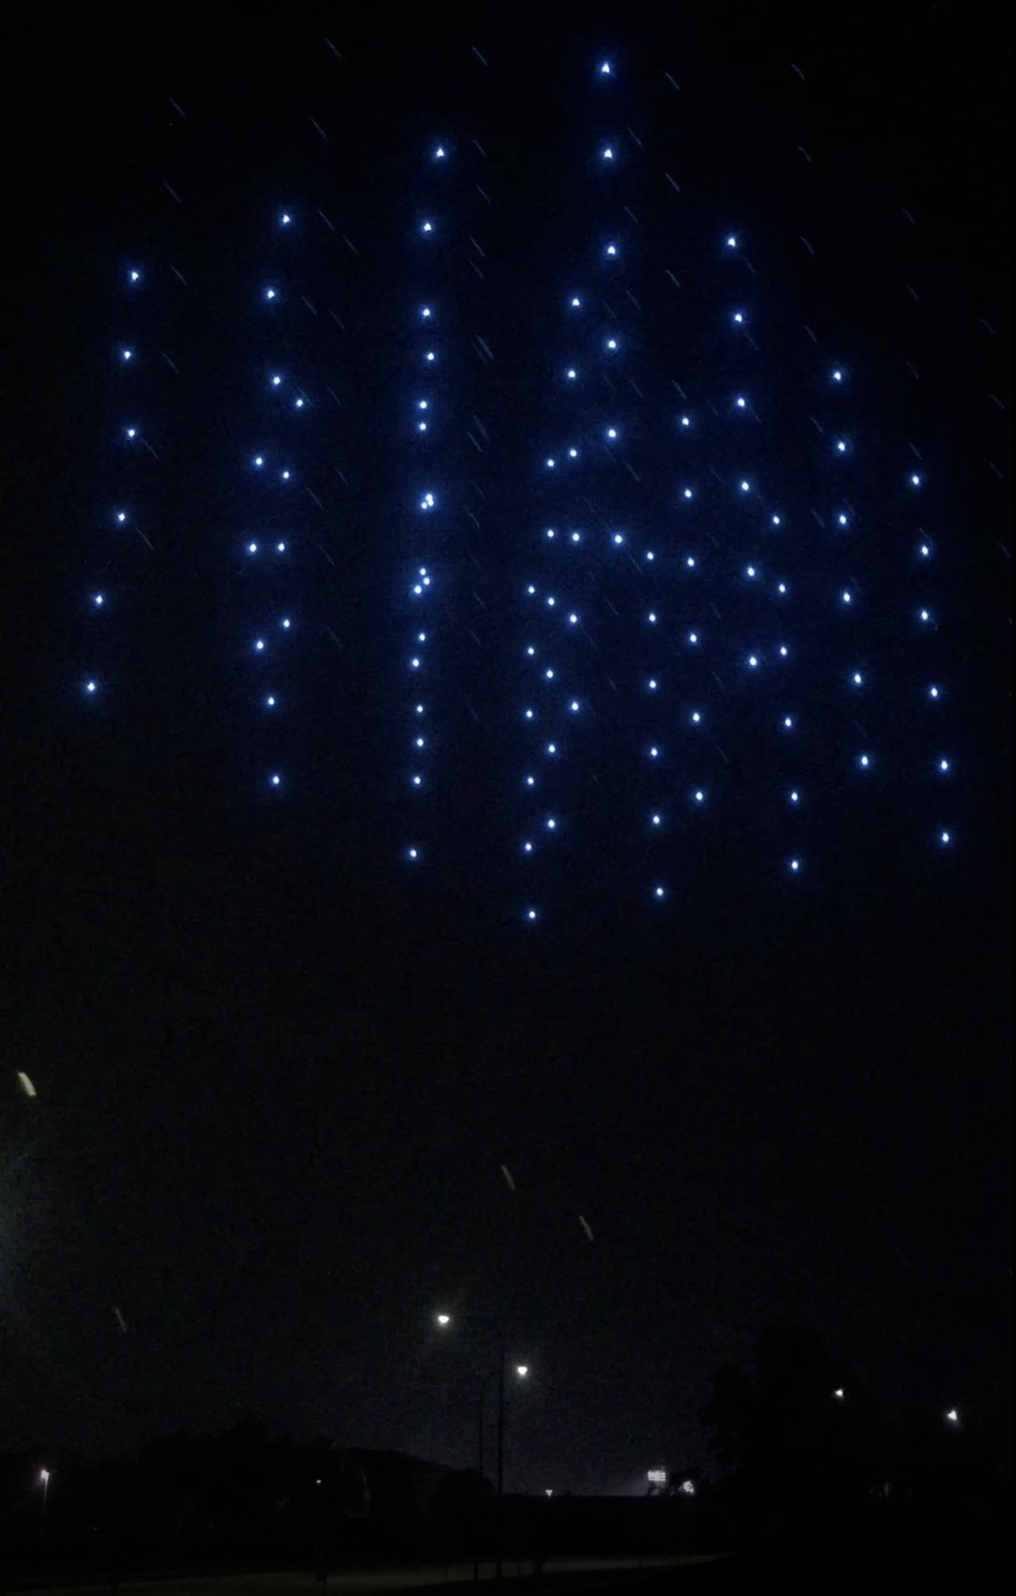
\includegraphics[width=\linewidth]{figs/firefly.png}
\end{minipage}
\begin{minipage}{0.55\columnwidth}
	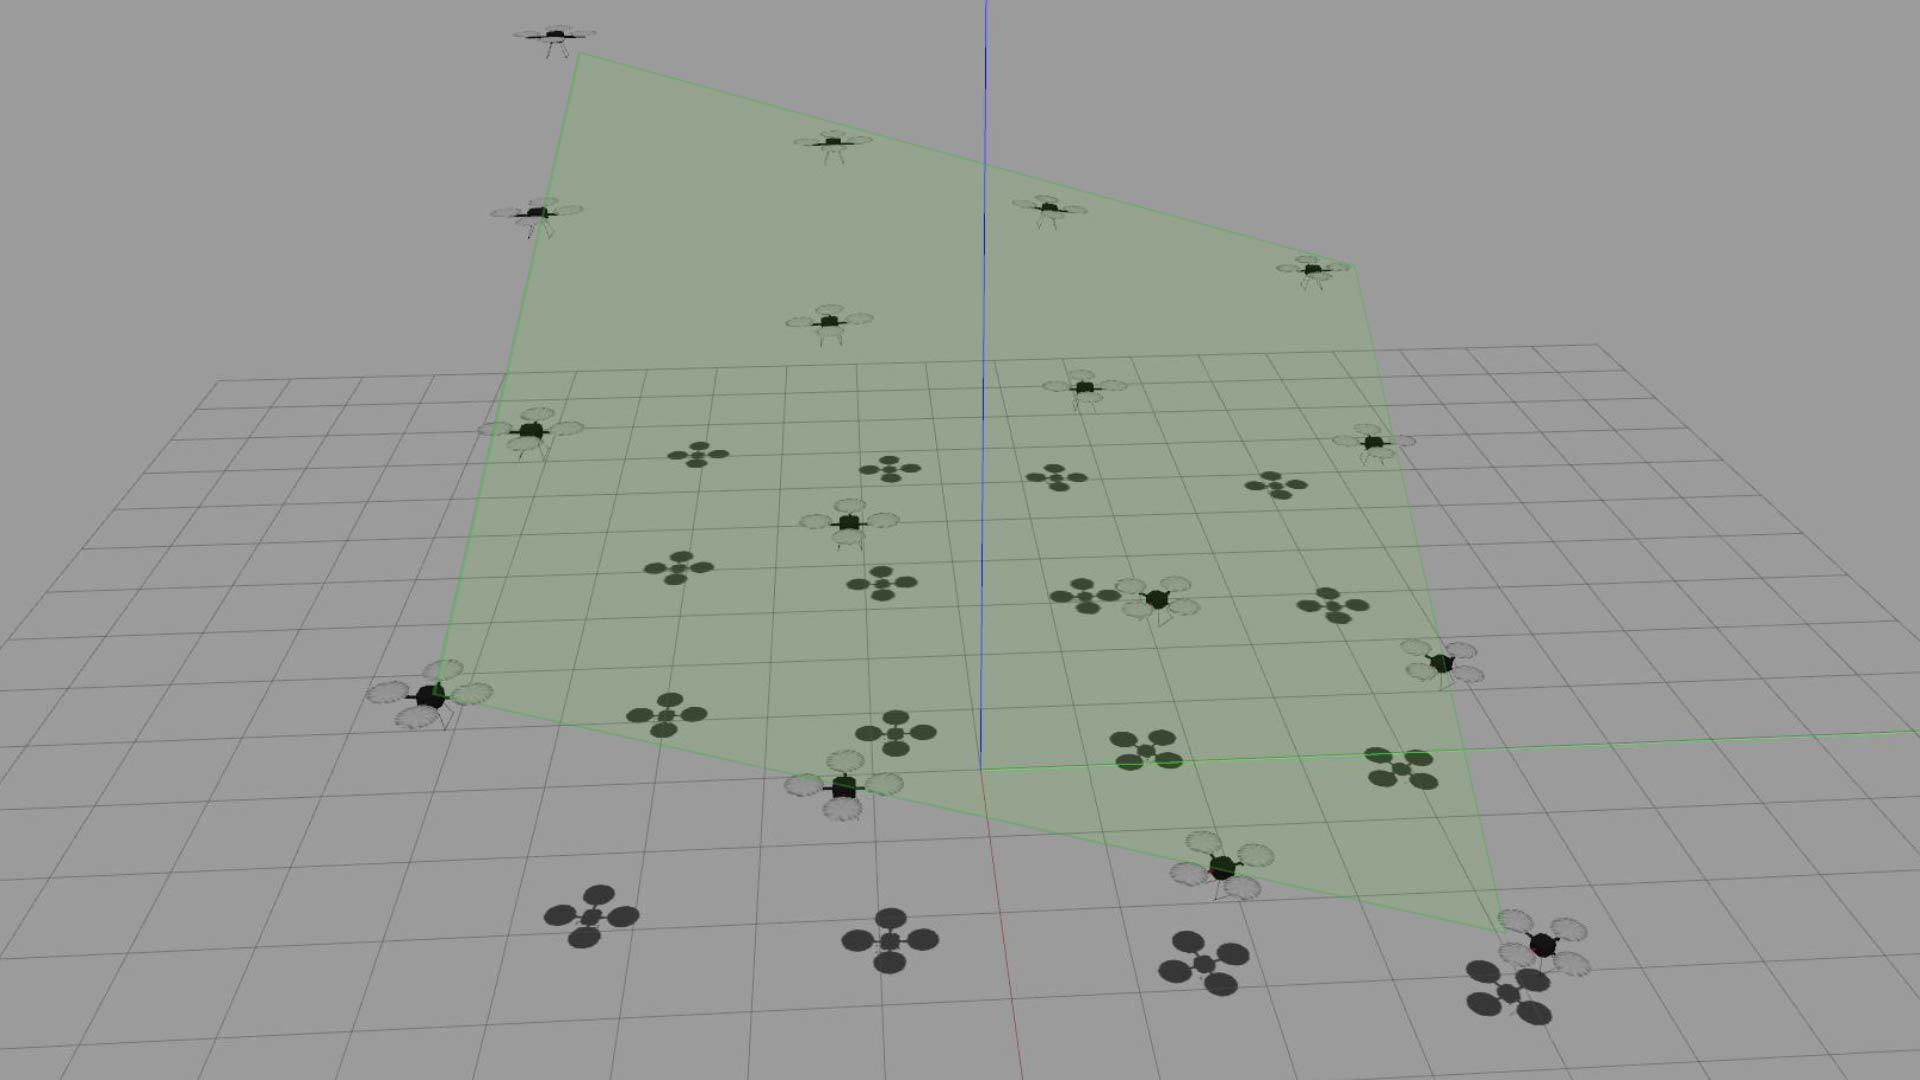
\includegraphics[width=\linewidth]{figs/shapeform_16.jpg}

	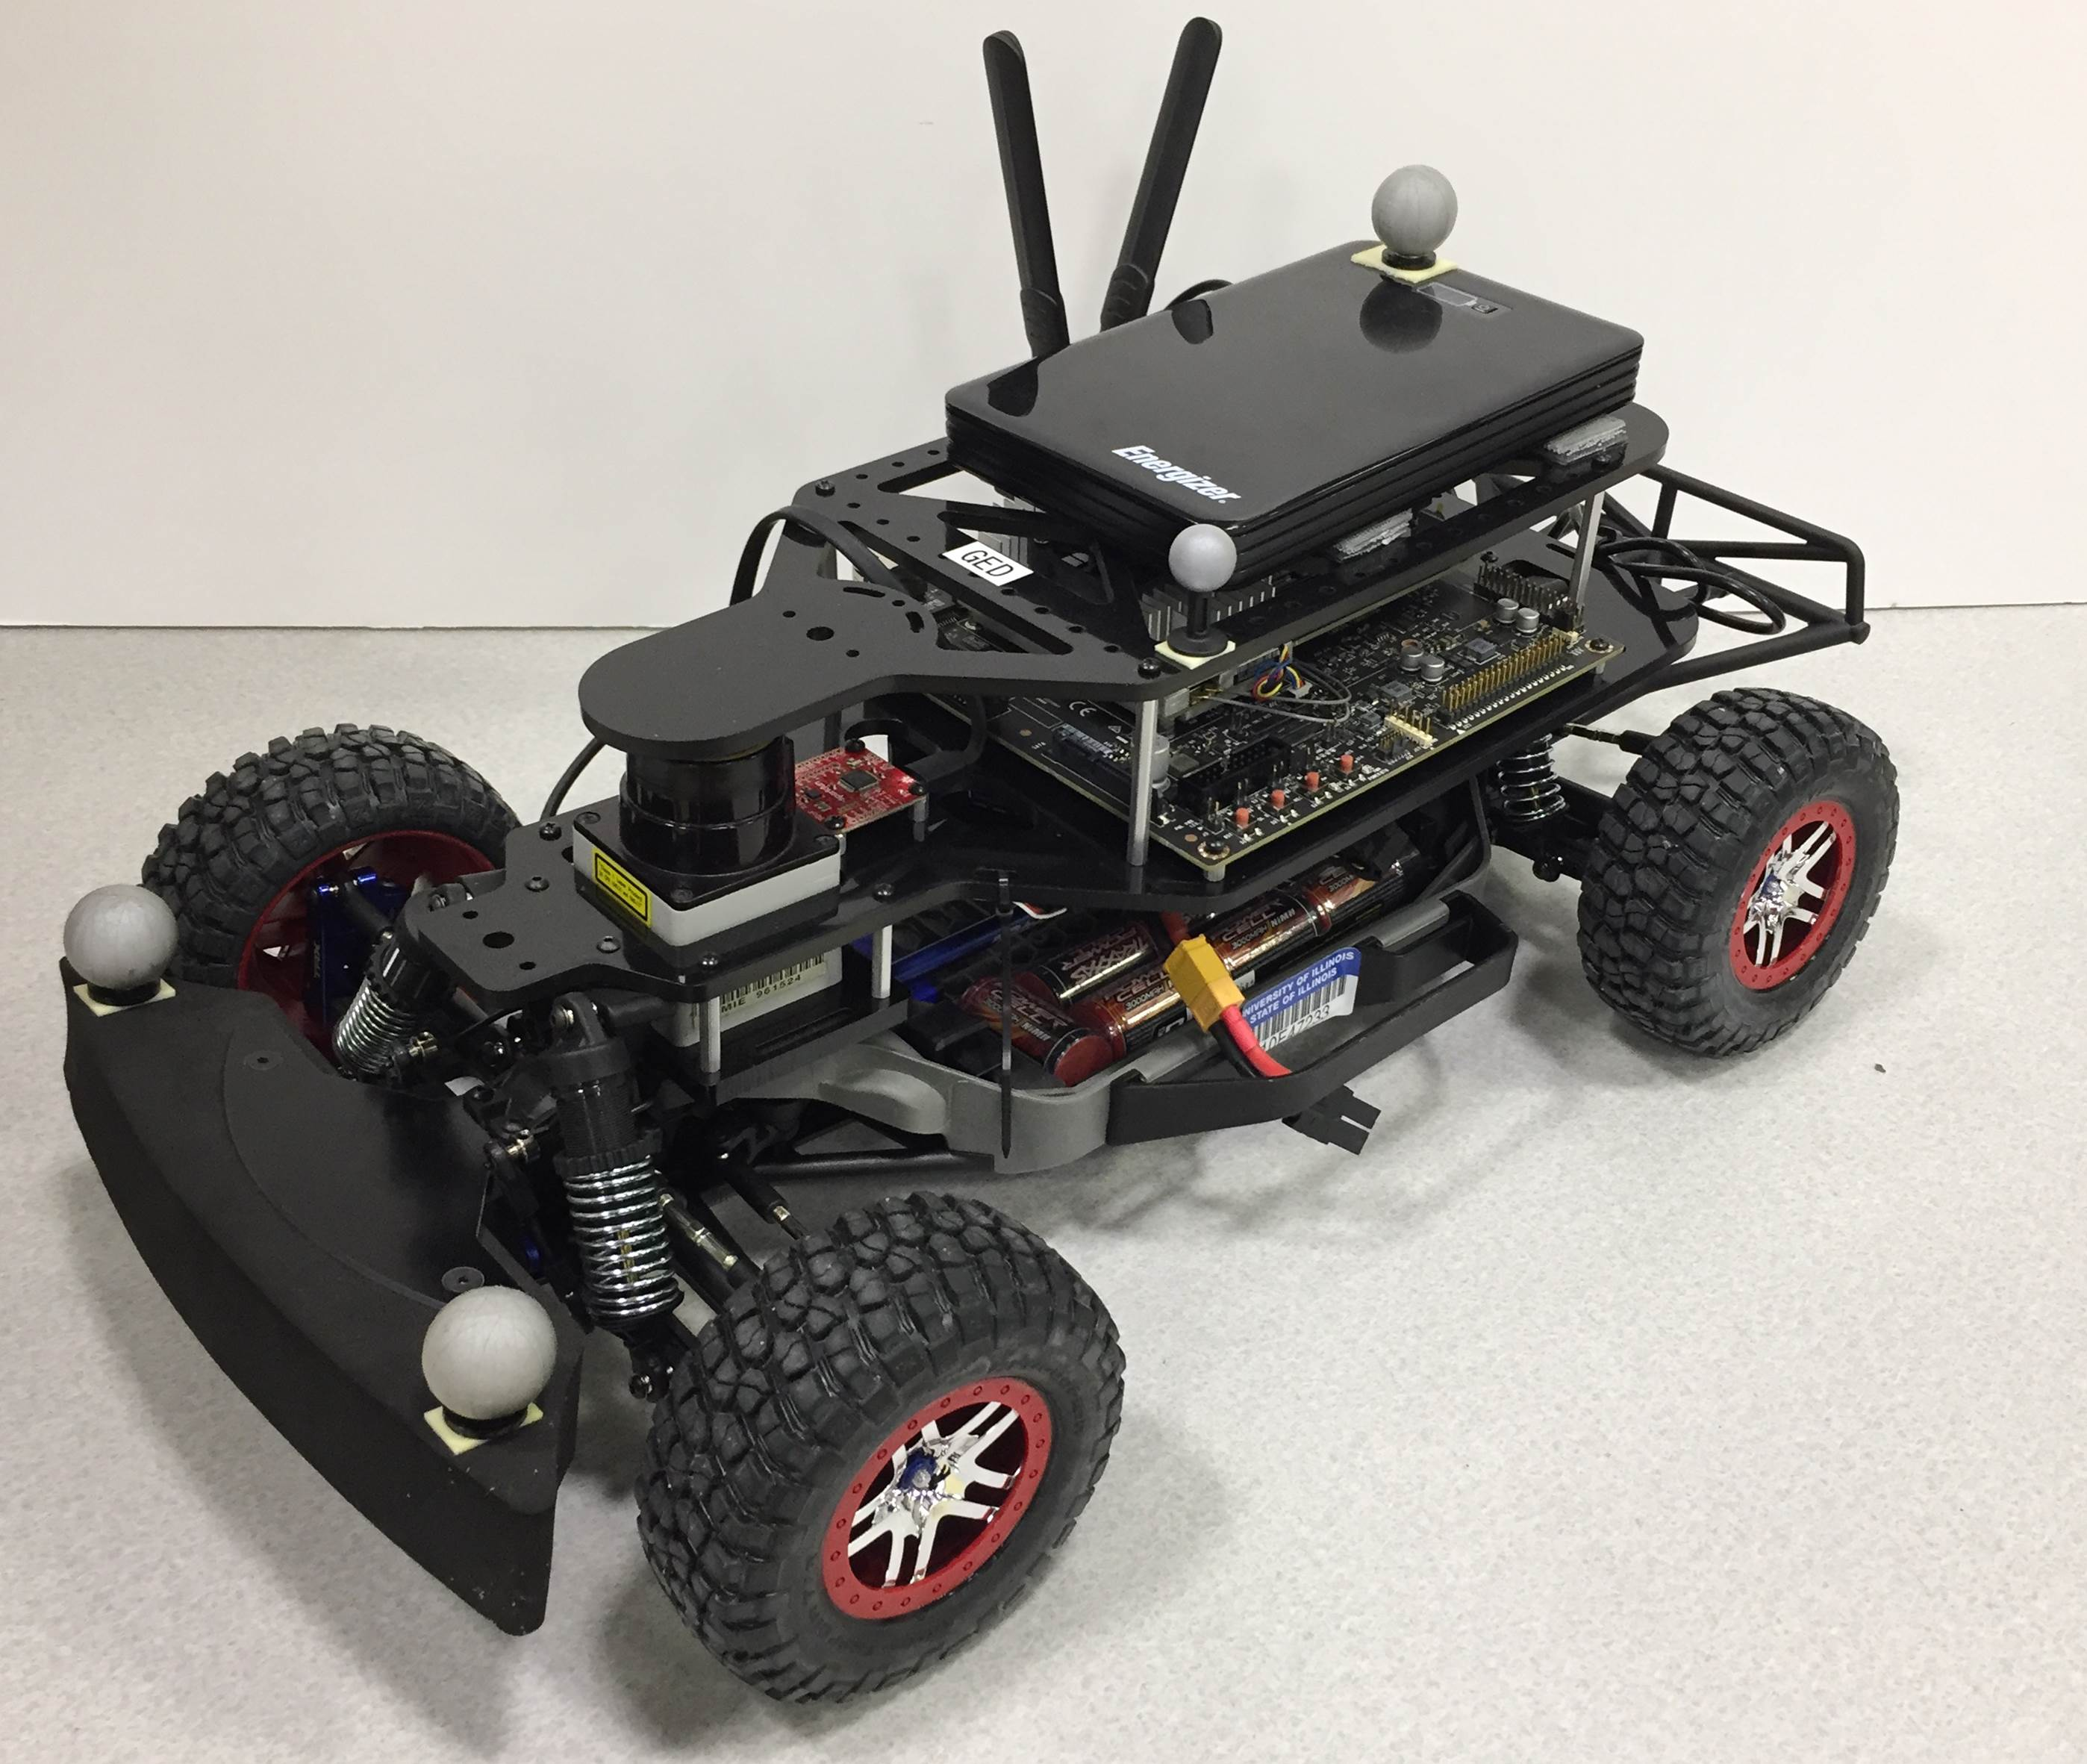
\includegraphics[width=0.42\linewidth]{figs/car.jpg}
	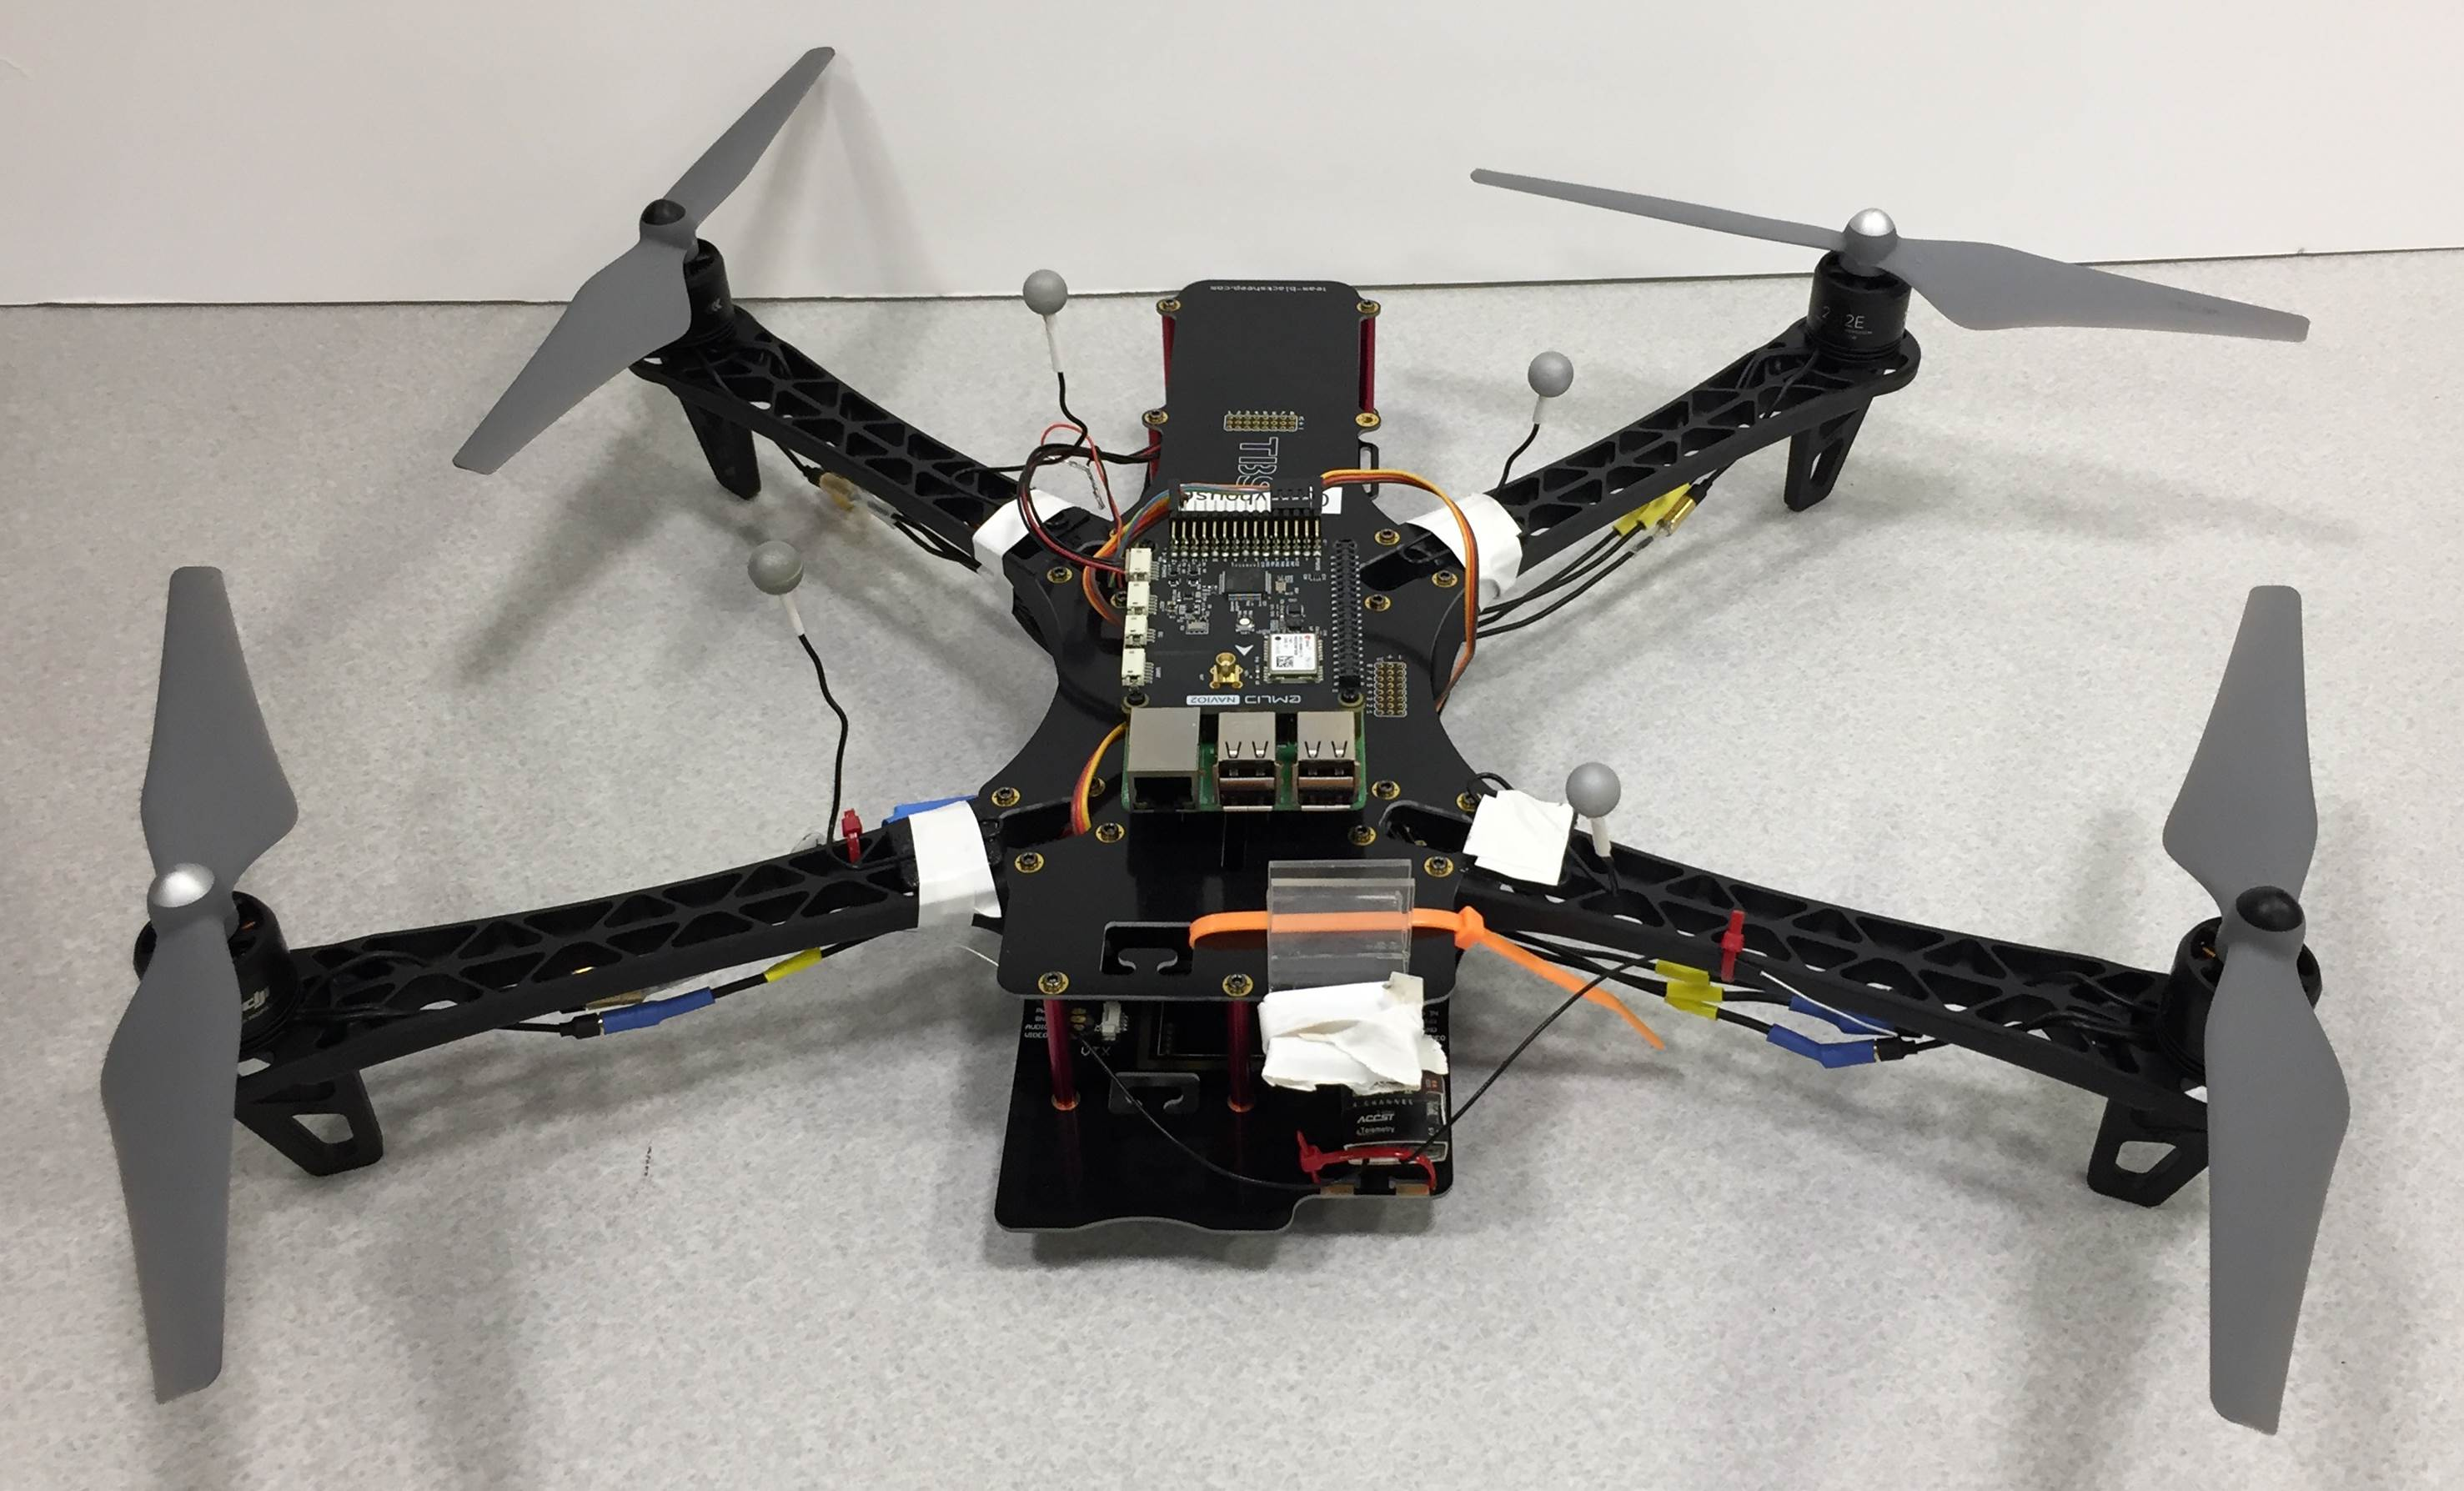
\includegraphics[width=0.56\linewidth]{figs/quad.jpg}
\end{minipage}%
	\caption{\small
        Swarm formation show by FireFly Inc. (\emph{Left}).
        Simulation of shape formation (\emph{Top Right}).
        Cars and quadcopters we can deploy and test $\lgname$ programs.\vspace{-5mm}}
    \label{fig:firefly}
\end{figure}
Programming languages like C\#, Swift, Python, and development tools like LLVM~\cite{llvm} have helped make millions of people, with diverse backgrounds, into mobile application developers, and open source software libraries like PyTorch~\cite{NEURIPS2019_9015} and Tensorflow~\cite{tensorflow2015-whitepaper} have propelled the surge in machine learning research and development. To a lesser degree, similar efforts in democratization of roboticsa are being made. Among existing robotics programming frameworks, ROS~\cite{ros} provideS hardware abstractions, device drivers, messaging protocols, many common library functions and has become widely used. Libraries such as PyRobot~\cite{pyrobot2019} and PythonRobotics~\cite{sakai2018pythonrobotics} provide hardware-independent implementations of common functions for physical manipulation and navigation of individual robots. Nevertheless, it requires significant effort and time of the order of weeks to develop, simulate, and debug a new application for a single mobile robot---not including the effort to build the robot hardware. The required effort grows quickly for distributed and heterogeneous systems, as none of the existing robotics libraries provide either (a) support for distributed  coordination, or (b) easy portability of code across different platforms. Further, available domain specific languages (DSL) for robotics are tightly coupled with platforms, and they combine low-level sensing, communication, and control tasks with the application-level logic. This tight-coupling and the attendant lack of abstraction hinders application development on all fronts---portability, code reuse, and verification and validation (V\&V).

In particular, formal reasoning about a collection of robots communicating, coordinating, and interacting with a physical environment is complexified by cyber-physical interactions. Correctness under concurrency and asynchrony are prominent research problems in distributed computing. Correctness under noise, disturbances, and imprecise platform (plant) models is studied intensively by roboticists and control theorists. The analysis techniques from these communities are based on very different formal models and mathematics, and both would be necessary  to provide satisfactory safety guarantees for  distributed robotic applications. Further, mathematical models and formal analysis techniques at the application design level often do not take into account the gap between design and implementation. 

One of the motivations for my thesis is {\em not\/} to combine all of the above in an {\em all encompassing formalism\/}; but to create a language that separates the concerns of building a reliable distributed cyber-physical application to divide and conquer using existing analyses from both the robotics and formal methods communities. The other, is to empirically  demonstrate the feasibility of implementing such a language, and narrow the gap between mathematical modelling and implementation as much as possible. 

\paragraph*{Contributions}
I have designed a formal semantics of a high level language~\cite{ghosh_language_2018}, which provides several abstractions for separation of platform-dependent and independent concerns, and implemented an executable semantics of the same in the \K semantic framework. \lgname applications can be simulated or deployed using the CyPhyHouse toolchain, which includes a compiler for \lgname, a high fidelity simulator, deployment and monitoring tools~\cite{ghosh2019cyphyhouse}. I have also developed a tool, using a verification approach that requires defined port assumptions, proof
obligations to provide guarantees which can be posed as inductive invariants~\cite{pldisub}. While I have only considered safety properties or invariants in \lgname applications, my work on verifying self-stabilisation of distributed algorithms~\cite{ghoshforte2015} provides an insight into extending the aforementioned verification approach to progress properties.







%- Koord compiler generated code,
%- Application code is less than 50 lines in Koord,
%- Reconfiguration, heterogeneity---configuration file.
%- First demonstration of .... distributed task allocation on HW?

%How long is the platform independent application code? Code can be simulated. We developed F1/10 and drone HW, and deployed it. This involved development of platform specific model-predictive controllers for F11/10 vehicles and aerial drones. Experiments.
